% !TEX root = ../main.tex
\section{Data Analysis}
\label{13::data_analysis}
    The first section describes a C program developed by the author to perform the analysis in this thesis.
    The second section discusses the DIS kinematics, which define the cuts made to the data.
    The third section provides detailed information about the approach used to include the sampling fraction in the analysis.
    Finally, the last section describes the simulations produced and the acceptance study conducted based on them.

    % !TEX root = ../main.tex
\subsection{\texttt{clas12-rge-analysis}}
\label{13.10::clas12_rge_analysis}
    To perform the acceptance analysis reported in this thesis, the author developed an extensive C/C++ program that runs on the ROOT library.
    The purpose of this program is not only to conduct the analysis described in this thesis but also to be used for RG-E analysis in general.
    The program and its source code are freely available under the GNU LGPLv3 license and can be accessed on GitHub at: \href{https://github.com/bleaktwig/clas12-rge-analysis}{github.com/bleaktwig/clas12-rge-analysis}.
    Issues and pull requests are welcomed, as they are crucial for maintaining the program and facilitating collaborative development in the repository.

    After compiling the program using \texttt{make}, five executables are obtained in the \texttt{bin} directory.
    The following sections provide a description of each executable.

    % !TEX root = ../main.tex
\subsubsection{\texttt{hipo2root}}
\label{sssec::hipo2root}
    CLAS12 reconstruction uses a custom data file named High-Performance Input Output (HIPO) format, developed by Gagik Gavalian \cite{chekanov2021}.
    The CLAS collaboration provides a set of tools to work with this format, allowing to read, write, and draw plots from HIPO files.
    Despite this, however, users at RG-E are much more familiar with the traditional ROOT files, and thus a conversion tool was developed.

    \texttt{hipo2root} filters through a HIPO file's data, and creates a ROOT file with pre-selected sections of storage, called banks.
    The selection of banks is based on data that is useful to RG-E analysis, and a user can easily add additional banks by editing the program's source files.
    The output of the executable is a ROOT file containing the selected banks as trees, a standard ROOT array-like variable.

    It's manual entry is:
    \begin{lstlisting}
Usage: hipo2root [-hfn:w:] infile
 * -h         : show this message and exit.
 * -f         : set this to true to process FMT::Tracks bank. If this is set
                and FMT::Tracks bank is not present in the HIPO file, the
                program will crash.
 * -n nevents : number of events.
 * -w workdir : location where output root files are to be stored. Default
                is root_io.
 * infile     : input HIPO file. Expected format is <text>run_no.hipo.

Convert a file from hipo to root format. This program only conserves the banks that are useful for RG-E analysis, as specified in the `lib/rge_hipo_bank.h` file. It's important for the input hipo file to specify the run number at the end of the filename (`<text>run_no.hipo`), so that `hipo2root` can get the beam energy from the run number.

Since simulation files don't have a run number, we use a convention for specifying the beam energy. For this files, the filename should be `<text>999XXX.hipo`, where `XXX` is the beam energy used in the simulation in [0.1*GeV].
    \end{lstlisting}

    % !TEX root = ../main.tex
\subsubsection{\texttt{extract\_sf}}
\label{sssec::extract_sf}
    Some analysis from CLAS12 is needed to obtain the sampling fraction of the detector's calorimeters.
    This is done by the \texttt{extract\_sf} executable, which uses the particles' momenta and deposited energy.
    The exact methodology and results obtained are discussed in section \ref{ssec::sampling_fraction}.

    The manual entry of the program is:
    \begin{lstlisting}
Usage: extract_sf [-hn:w:d:] infile
 * -h         : show this message and exit.
 * -n nevents : number of events
 * -w workdir : location where output root files are to be stored. Default
                is root_io.
 * -d datadir : location where sampling fraction files are stored. Default
                is data.
 * infile     : input ROOT file. Expected file format: <text>run_no.root.

Obtain the EC sampling fraction from an input file. An alternative to using this program is to fill the output file corresponding to the studied run (by default stored in the `data` directory) with the data obtained from [CCDB](https://clasweb.jlab.org/cgi-bin/ccdb/versions?table=/calibration/eb/electron_sf). The function used to fit the data is

[0]*Gaus(x,[1],[2]) + [3]*x*x + [4]*x + [5]

where *[0]* is the amplitude of the Gaussian, *[1]* and *[2]* its mean and sigma, and *[3]*, *[4]*, and *[5]* the *p0*, *p1*, and *p2* used to fit the background.

The output of the program is the `sf_params_<run_no>.txt`, which contains a table with the sampling fractions and their errors. The table is formatted like the one at CCDB, as in

         | sf0     sf1     sf2     sf3     sfs1    sfs2    sfs3    sfs4
---------+-----------------------------------------------------------------
sector 1 | %011.8f %011.8f %011.8f %011.8f %011.8f %011.8f %011.8f %011.8f
sector 2 | %011.8f %011.8f %011.8f %011.8f %011.8f %011.8f %011.8f %011.8f
sector 3 | %011.8f %011.8f %011.8f %011.8f %011.8f %011.8f %011.8f %011.8f
sector 4 | %011.8f %011.8f %011.8f %011.8f %011.8f %011.8f %011.8f %011.8f
sector 5 | %011.8f %011.8f %011.8f %011.8f %011.8f %011.8f %011.8f %011.8f
sector 6 | %011.8f %011.8f %011.8f %011.8f %011.8f %011.8f %011.8f %011.8f
    \end{lstlisting}

    % !TEX root = ../main.tex
\subsubsection{\texttt{acc\_corr}}
\label{sssec::acc_corr}
    The \texttt{acc\_corr} executable is used to count the number of thrown and simulated events from two different ROOT files.
    Based on the program's input, it separates the data into appropriate 5-dimensional bins, counts the entries for all available particles in the generated file, and exports the results into a text file.
    The results and plots presented in section \ref{ssec::acceptance_correction} were generated using the data obtained from this program.

    The manual entry of the program is:
    \begin{lstlisting}
Usage: acc_corr [-hq:n:z:p:f:g:s:d:FD]
 * -h         : show this message and exit.
 * -q ...     : Q2 bins.
 * -n ...     : nu bins.
 * -z ...     : z_h bins.
 * -p ...     : Pt2 bins.
 * -f ...     : phi_PQ bins (in degrees).
 * -g genfile : generated events ROOT file.
 * -s simfile : simulated events ROOT file.
 * -d datadir : location where sampling fraction files are found.
                Default is data.
 * -F         : flag to tell program to use FMT data instead of DC data
                from the simulation file.
 * -D         : flag to tell program that generated events are in
                degrees instead of radians.

Get the 5-dimensional acceptance correction factors for *Q2*, *nu*, *z_h*, *Pt2*, and *phi_PQ*. For each optional argument, an array of doubles is expected. The first double will be the lower limit of the leftmost bin, the final double will be the upper limit of the rightmost bin, and all doubles between them will be the separators between each bin.

The output will be written to the `acc_corr.txt` file, by default in the `data` directory, which is formatted to make it easy to read by the `draw_plots` program:
* First line contains five integers; the size of each of the five binnings.
* The next five lines are each of the binning schemes, in order *Q2*, *nu*, *z_h*, *Pt2*, and *phi_PQ*.
* The following line contains one integer which is the size of the list of PIDs, followed by a line containing each of these PIDs.
* Finally, a number of lines equal to the number of PIDs follows. Each line contains a list of the bins, ordered as `[Q2][nu][z_h][Pt2][phi_PQ]`.
    \end{lstlisting}

    % !TEX root = ../main.tex
\subsubsection{\texttt{make\_ntuples}}
\label{13.14::make_ntuples}
    This executable operates on one or more files generated by \texttt{hipo2root} and produces a ROOT file that contains a set of \texttt{ntuples} relevant to the analysis.
    Furthermore, based on the specific requirements of this thesis' analysis, the executable generates two sets of \texttt{ntuples}.
    Both sets have the same \texttt{ntuple} format, but the former utilises only DC tracking data while the latter incorporates both DC and FMT tracking data.

    \begin{table}[b]
        \begin{tabularx}{240pt}{Xllllll}
            \multicolumn{7}{c}{\textit{Particle Identification Truth}} \\
            \toprule
                     & $e$      & $\pi$ & $K$  & $p$  & $n$  & $\gamma$ \\
            \midrule
            $e$      & 1.00     &       &      &      &      &          \\
            $\pi$    &          & 1.00  & 0.09 & 0.02 &      &          \\
            $K$      &          &       & 0.91 &      &      &          \\
            $p$      &          &       &      & 0.98 &      &          \\
            $n$      &          &       &      &      & 1.00 &          \\
            $\gamma$ &          &       &      &      &      & 1.00     \\
            \bottomrule
        \end{tabularx}
        \caption[Particle identification matrix for the FD]
        {Particle identification matrix for the FD.
        The rows show the PID assigned by reconstruction while the columns the one assigned by the \texttt{make\_ntuples} program.
        The diagonal elements are correctly identified, while the off-diagonal elements are misidentified.}
        \label{tab::13.14::make_ntuples_pid}
    \end{table}

    For each event, the program executes the following algorithm:

    \begin{enumerate}
        \item
            First, the program identifies the TOF of the trigger electron.
            The hits of the trigger electron in the FD scintillators and FD calorimeters are listed in order of priority based on the precision of each detector's TOF measurement.
            The detectors are prioritised as follows: FTOF panel-1b, FTOF panel-1a, FTOF panel-2, PCAL, ECIN, and ECOU, as described in Section \ref{11.210::forward_detector}.
            Next, the program iterates over the list of hits, extracting the TOF value from the earliest hit in the most precise available layer.

        \item
            Next, for each available track, two particle objects are instantiated.
            These objects contain the relevant data for the particle, including its vertex position, vertex momentum, charge, beta, and the CLAS12 sector through which it passed.
            The first object corresponds to the tracking data obtained from the DC, while the second object incorporates both the DC and the FMT tracking data.
            The assignment of the particle's PID will be carried out later in the process.

        \item
            The program computes and stores the particle's deposited energy in the calorimeters.
            This involves summing up the energy deposited by all the hits associated with the particle's track for each calorimeter.

        \item
            The program counts the number of produced photoelectrons in the HTCC and LTCC for the particle.
            Furthermore, the particle's TOF is computed using the same procedure as the one employed for the trigger electron's TOF, considering the hits in the detectors prioritised by their precision.

        \item
            The program assigns the Particle Identification PID to the particle.
            The process is very similar to the PID assignment in reconstruction, as described in Section \ref{11.230::offline_reconstruction}.
            However, the assigned PID is not directly used in order to allow users to modify parameters and define new criteria for the PID assignment.

            Although this process typically yields the same results as reconstruction, there is a slight error in the PID assignment.
            This error is presented in Table \ref{tab::13.14::make_ntuples_pid}.
            As shown in the table, some kaons and protons are misidentified as pions, but the degree of misidentification is not significant.
            Apart from that, all identifications are accurate.

        \item
            Finally, two \texttt{ntuples} objects are created: one for the particle generated from the DC tracking data and another for the particle generated from both the DC and FMT data.
            These \texttt{ntuple} objects are then saved in an output file, which can be used directly for analysis or processed by the \texttt{draw\_plots} program discussed in the next section.
    \end{enumerate}

    \pagebreak

    The manual entry of the program is:
    \begin{lstlisting}
Usage: make_ntuples [-hDf:cn:w:d:] infile
 * -h         : show this message and exit.
 * -D         : activate debug mode.
 * -f fmtlyrs : define how many FMT layers should the track have hit.
                Options are 0 (tracked only by DC), 2, and 3. If set to
                something other than 0 and there is no FMT::Tracks bank
                in the input file, the program will crash. Default is
                0.
 * -c         : apply FMT geometry cut on data.
 * -n nevents : number of events.
 * -w workdir : location where output root files are to be stored.
                Default is root_io.
 * -d datadir : location where sampling fraction files are. Default is
                data.
 * infile     : input ROOT file. Expected file format:
                <text>run_no.root`.

Generate ntuples relevant to SIDIS analysis based on the reconstructed variables from CLAS12 data. The output of the program is the `ntuples_<run_no>.root` file, which contains all relevant ntuples for RG-E analysis. This file can be studied directly in root or through the `draw_plots` program.
    \end{lstlisting}

    % !TEX root = ../main.tex
\subsubsection{\texttt{draw\_plots}}
\label{sssec::draw_plots}
    This executable is included so that the user doesn't have to re-write similar code regularly to obtain plots.
    Operating \texttt{draw\_plots} is fairly simple: after running the program, the user must answer a set of question to define the various attributes related to the plots.
    This includes cuts and corrections to apply, binning setup, and, naturally, the variables in the plots.
    Unless otherwise specified, the plots included in section \ref{sec::resultsandconclusions} were produced using this executable.

    The executable's manual entry is:
    \begin{lstlisting}
Usage: draw_plots [-hp:cn:o:a:w:] infile
 * -h          : show this message and exit.
 * -p pid      : skip particle selection and draw plots for pid.
 * -c          : apply all cuts (general, geometry, and DIS) instead of
                 asking which ones to apply while running.
 * -n nentries : number of entries to process.
 * -o outfile  : output file name. Default is plots_<run_no>.root.
 * -a accfile  : apply acceptance correction using acc_filename.
 * -A          : get acceptance correction plots without applying acceptance
                 correction. Requires -a to be set.
 * -w workdir  : location where output root files are to be stored. Default
                 is root_io.
 * infile      : input file produced by make_ntuples.\n

Draw plots from a ROOT file built from `make_ntuples`. File should be named `<text>run_no.root`. This tool is built for those who don't enjoy using root too much, and should be able to get most basic plots needed in SIDIS analysis.
    \end{lstlisting}


    % !TEX root = ../main.tex
\subsection{Cuts}
\label{ssec::cuts}
    In order to enhance the relevance of particles for the analysis presented in this work, three types of cuts are applied:
    \begin{itemize}
        \item
            General cuts:
            These cuts are designed to exclude poorly reconstructed particles.
        \item
            Geometry cuts:
            These cuts define the region from which the reconstruction data is considered valid and useful for the analysis.
        \item
            DIS cuts:
            These cuts narrow down the analysis region to focus specifically on DIS.
    \end{itemize}
    By applying these cuts, the analysis can be focused on particles that meet the criteria for good reconstruction, fall within the desired geometry range, and are relevant to the DIS process.

    % !TEX root = ../main.tex
\subsubsection{General Cuts}
\label{sssec::general_cuts}
    For this analysis, only two cuts are considered as ``general''.
    The first cut involves filtering out particles with PID values of 0 or 45.
    In CLAS12 reconstruction, these specific PID values are assigned to particles whose identification could not be successfully determined.

    The second cut aims to exclude particles with imprecise tracking and is defined as follows:
    \begin{equation*}
        \frac{\chi^2}{\text{NDF}} < 15,
    \end{equation*}
    where $\chi^2$ represents the final result from the $\chi^2$-test used in the Kalman filter fit of the tracking algorithm, as described in section \ref{sssec::offline_reconstruction}.
    The term NDF denotes the number of degrees of freedom associated with this same fit.

    By applying these two cuts, particles with undetermined or uncertain identification (PID values of 0 or 45) and those with poor tracking precision (exceeding the specified $\chi^2$/NDF threshold) are excluded from the analysis.

    % !TEX root = ../main.tex
\subsubsection{Geometry Cuts}
\label{13.22::geometry_cuts}
    Three geometry cuts are derived to constrain the reconstructed particle's vertex position.
    The first two cuts ensure that the vertex is located along the beamline, while the third cut restricts it to the acceptance region of the FMT.

    The first cut guarantees that the vertex is close to the beamline and is defined as
    \begin{equation*}
        \sqrt{v_x^2 + v_y^2} < 4 \text{ cm},
    \end{equation*}
    where $v_x$ and $v_y$ represent the $x$ and $y$ coordinates of the vertex position, respectively.

    The second cut ensures that the vertex originates from the target and is given by
    \begin{equation*}
        -40 \text{ cm} < v_z < z_0 \text{ cm},
    \end{equation*}
    where $v_z$ corresponds to the $z$ coordinate of the vertex position, and $z_0$ represents the $z$ position of the first FMT layer.
    For the RG-F Spring 2020 run, $z_0 = 26.12$ cm.

    The third and final cut ensures that the vertex falls within the FMT acceptance region, as defined in Section \ref{12.42::geometry_effect}.
    It removes all particles whose $v_z$ and $\theta$ values lie outside the region bounded by the two lines defined by Equation \eqref{eq::12.42::fmt_geometry_cut}.

    % !TEX root = ../main.tex
\subsubsection{DIS Cuts}
\label{13.23::dis_cuts}
    Three DIS cuts are applied to the scattered electron to restrict the phase space to that of DIS.
    If the trigger electron fails to pass these cuts, all particles in the event are disregarded.

    The first cut is based on the invariant mass of the virtual photon, $Q^2$, and is defined as
    \begin{equation*}
        Q^2 > 1 \text{ GeV}^2,
    \end{equation*}
    where $Q^2$ is given by
    \begin{equation}
        Q^2 = 4E_bE'\sin^2(\theta_C/2).
        \label{eq::13.23::q2}
    \end{equation}
    Here, $E_b$ represents the beam energy, $E'$ is the energy of the scattered electron, and $\theta_C$ is the polar angle of the scattered electron.
    This cut ensures that the process falls within the DIS domain, as explained in Sections \ref{10.10::deep_inelastic_scattering} and \ref{10.12::parton_model}.

    The second cut is imposed on the squared mass of the hadronic final state, $W^2$, given by
    \begin{equation*}
        W^2 > 4 \text{ GeV}^2.
    \end{equation*}
    Here, $W^2$ is defined as
    \begin{equation*}
        W^2 = M^2 + 2M\nu - Q^2,
    \end{equation*}
    where $M$ represents the mass of the nucleon, and $\nu$ is the energy transferred by the lepton probe.
    The details of the virtual photon energy $\nu$ and its effects on this analysis are explained in Section \ref{10::physics_motivation}, and it is given by
    \begin{equation}
        \nu = E_b - E'.
        \label{eq::13.23::nu}
    \end{equation}
    This cut is applied to exclude nucleon resonances.

    \begin{figure}[b!]
        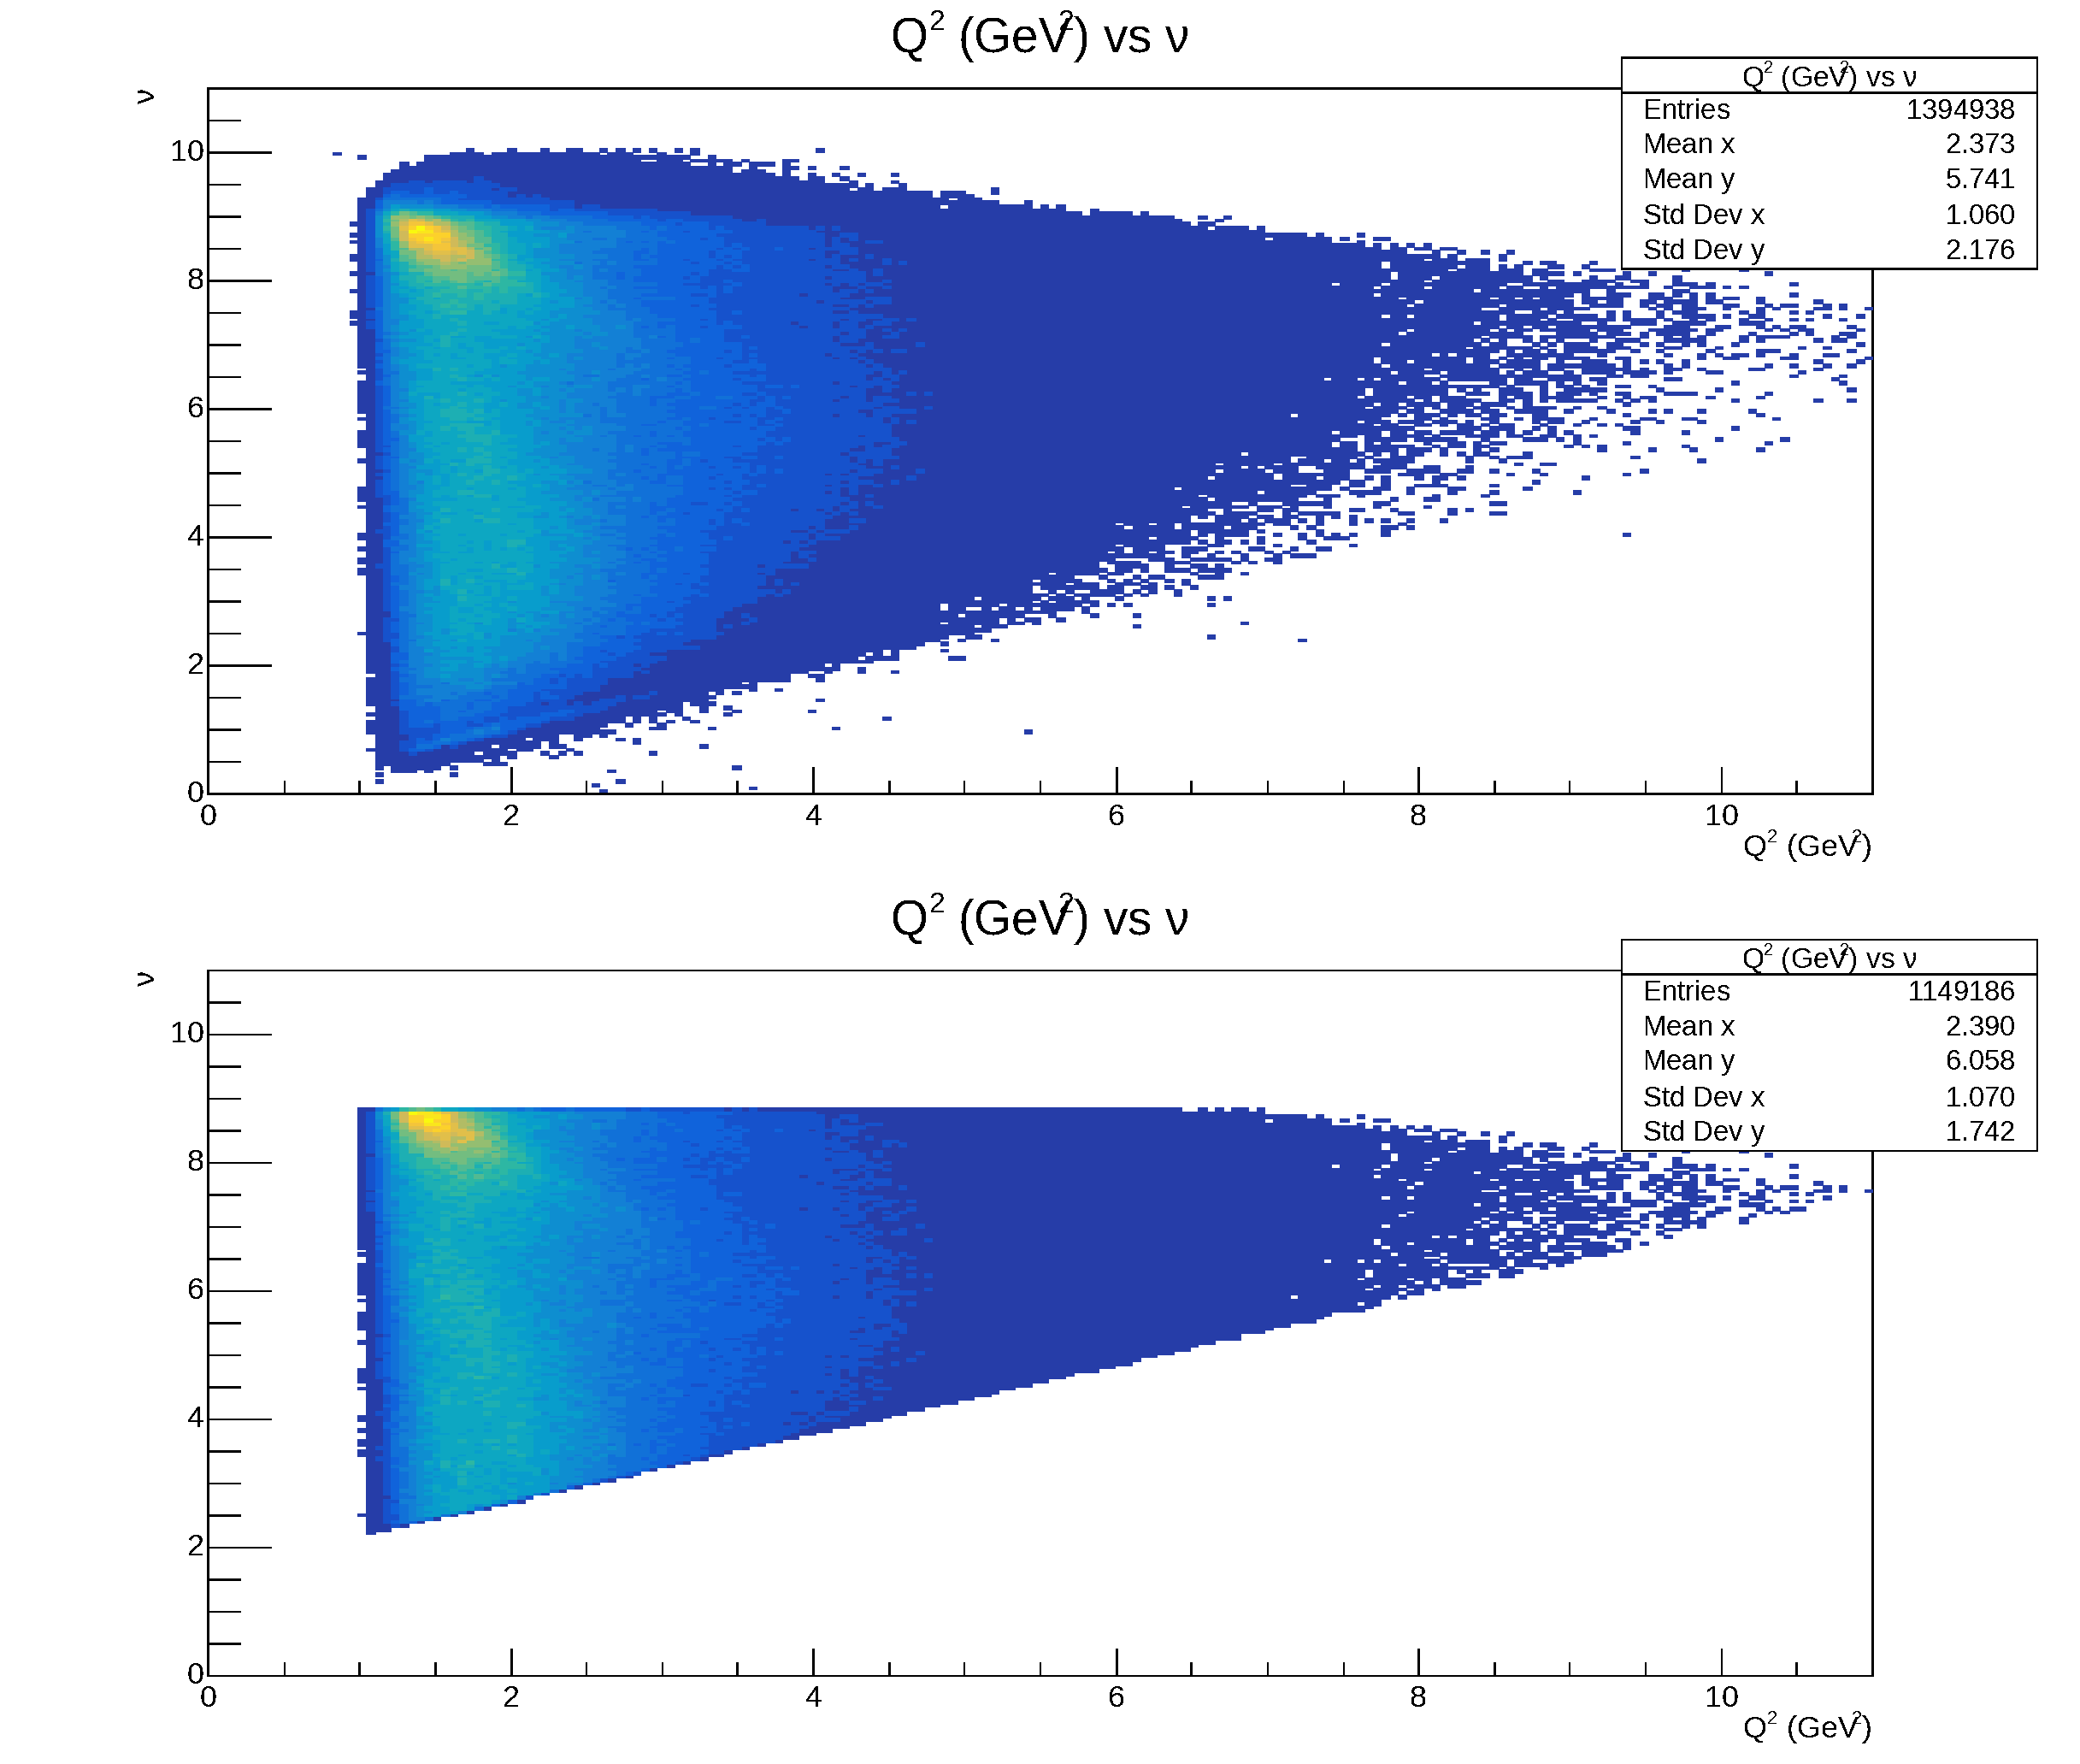
\includegraphics[width=\textwidth]{23q2_vs_nu.pdf}
        \caption[$Q^2$ vs. $\nu$ comparison]
        {$e^-$ $Q^2$ vs. $\nu$ before and after applying the $Q^2 > 1 \text{ GeV}^2$, $W^2 > 4 \text{ GeV}^2$, and $Y_b < 0.85$ cuts, run 12016.}
        \floatfoot{Source: Own elaboration, using the \href{https://github.com/bleaktwig/clas12-rge-analysis}{clas12-rge-analysis} software.}
        \label{fig::13.23::q2_vs_nu}
    \end{figure}

    Lastly, an additional cut is imposed on the Bjorken-Y ($Y_b$) of the scattered electron, given by
    \begin{equation*}
        Y_b < 0.85.
    \end{equation*}
    The Bjorken-Y ranges from 0 to 1 and is defined as
    \begin{equation*}
        Y_b = \frac{\nu}{E_b}.
    \end{equation*}
    This cut effectively mitigates the influence of extreme radiative effects, which occur when a substantial portion of the incident electron's energy is transferred to the scattered electron.

    The impact of these cuts on the $Q^2$ and $\nu$ of the scattered electron can be observed in plot \ref{fig::13.23::q2_vs_nu}.


    % !TEX root = ../main.tex
    \begin{figure}[b!]
        \centering\frame{
        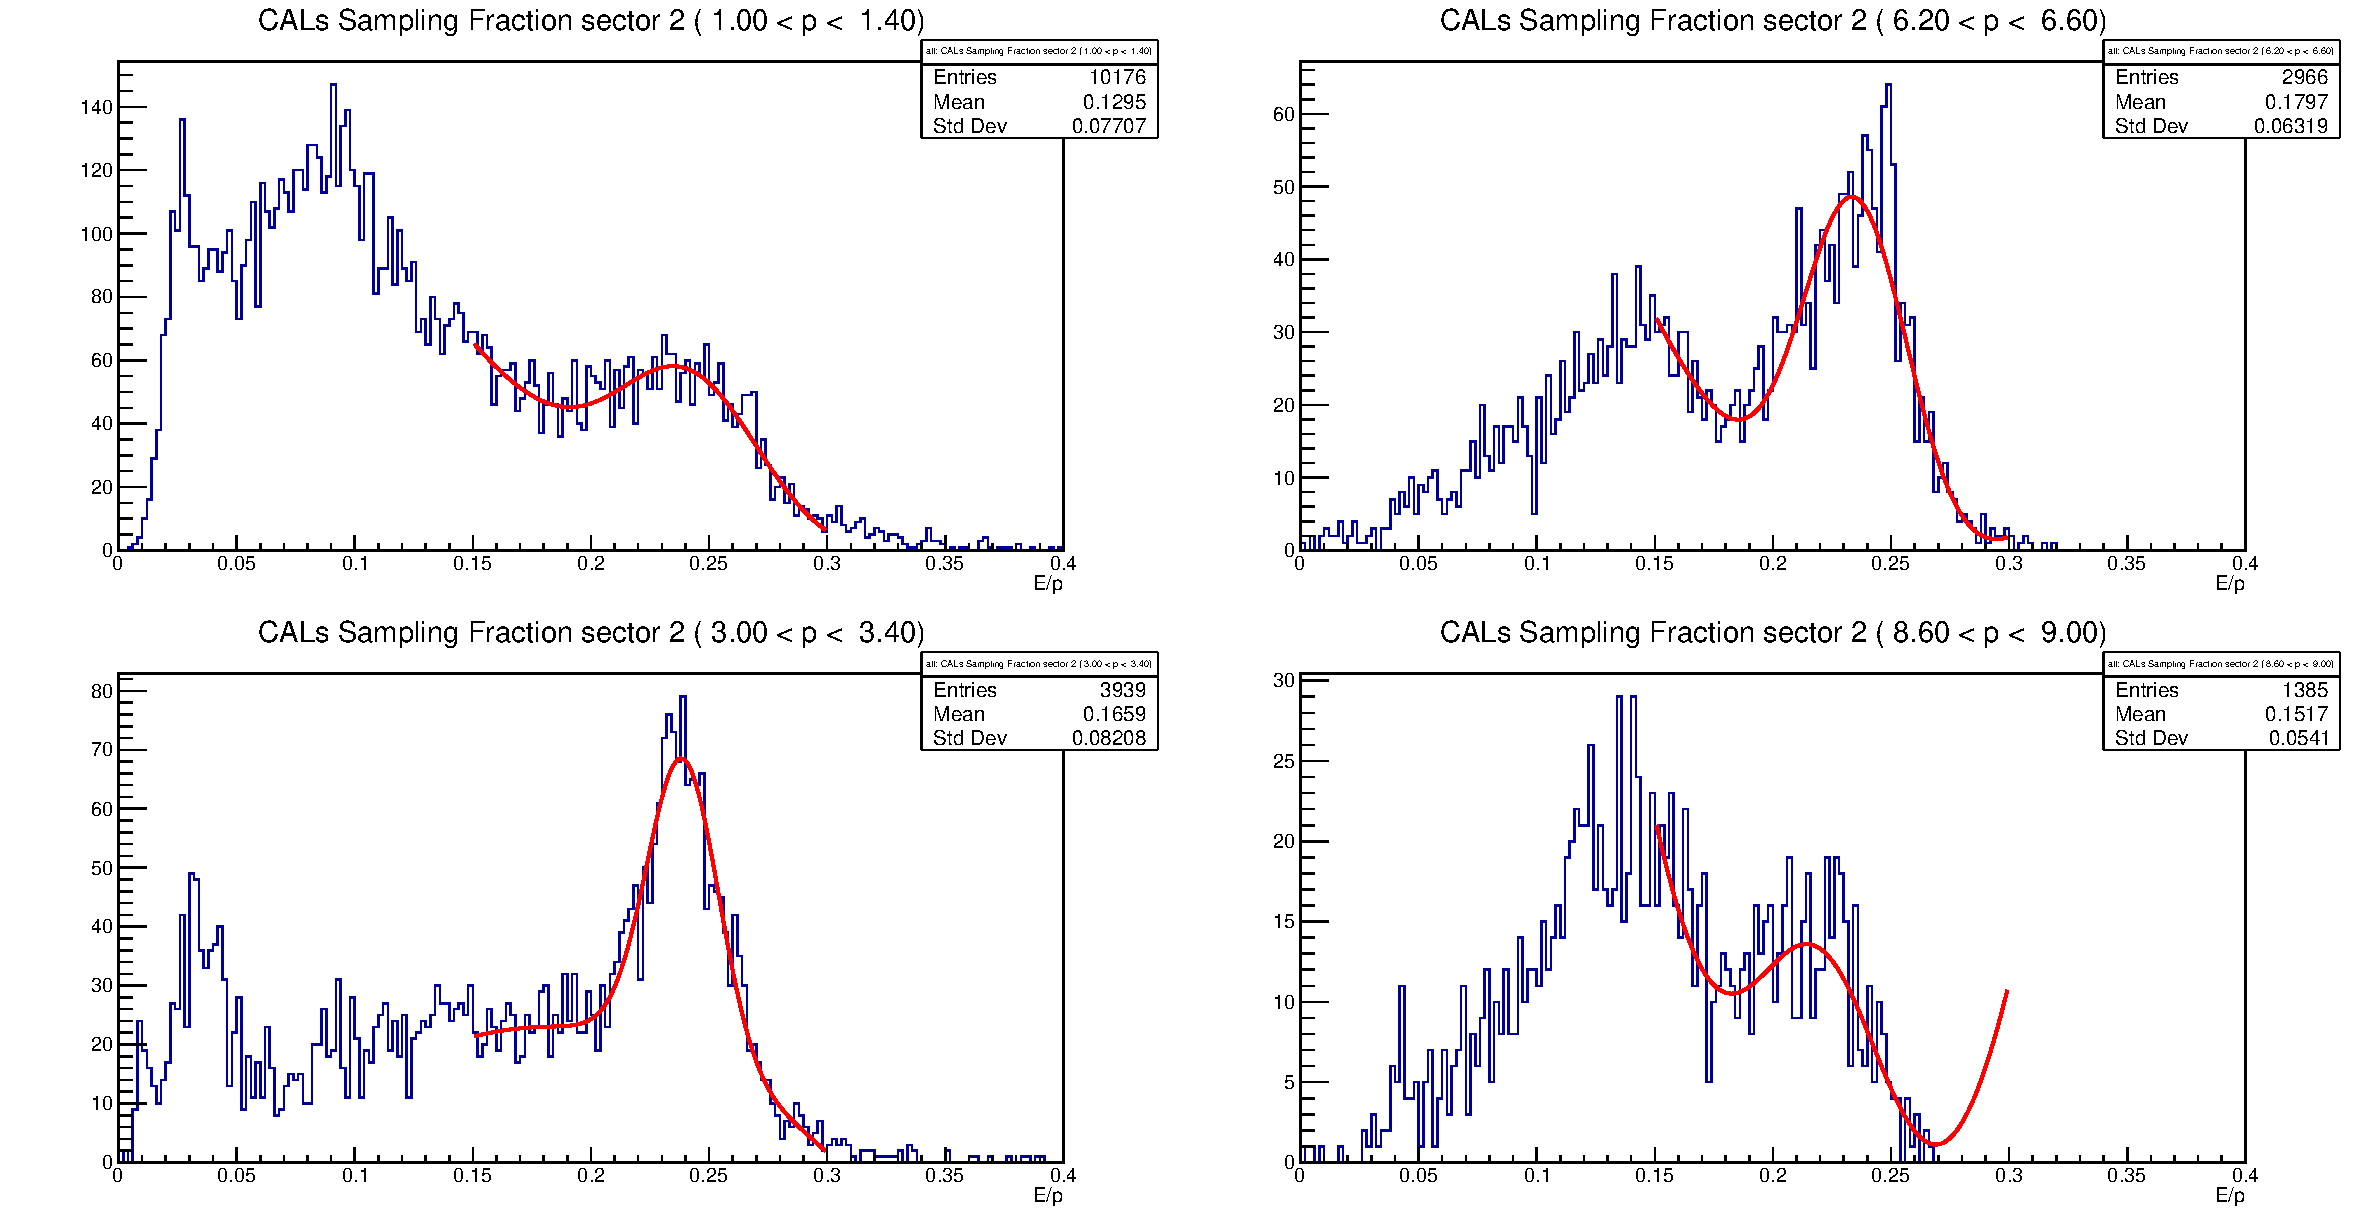
\includegraphics[width=\textwidth]{30sf_1d_plots.pdf}}
        \caption[Calorimeters $E/p$ plots]{Four $E/p$ plots describing the sum of the deposited energy per particle on all calorimeters (PCAL, ECIN, and ECOU).
        The particles' momentum is obtained from tracking and the event builder.
        As can be seen in the northwest and the southeast plots, the corner bins -- $1.00$ to $1.40$ and $8.60$ to $9.00$ GeV respectively -- are not very reliable.
        Source: Own elaboration, using the \hyperlink{github.com/bleaktwig/clas12-rge-analysis}{clas12-rge-analysis} software.}
        \label{fig::sf_1d}
    \end{figure}

\subsection{Sampling Fraction}
\label{ssec::sampling_fraction}
    The energy deposited by electrons in the active area of the calorimeters is a fraction of their total energy, $E_\text{tot}$.
    This value is proportional to their momentum, $P$, for energies above a few hundred MeV.
    Heavier particles, due to their reduced penetration capabilities, tend to lose an amount of energy independent of their momentum.
    The electron sampling fraction measures the amount of energy lost depending on the momentum of a particle.
    This allows for both the measurement of the electron's energy and the differentiation of electrons from other particles \cite{wigmans2000}.

    To obtain the sampling fraction, the hits of each calorimeter by itself (PCAL, ECIN, and ECOU) are separated into arrays, with an additional array containing the union of the other three.
    Then, these arrays of hits are separated into 20 momentum bins.
    Each bin has a size of 0.4 GeV, starting at 1.0 GeV and ending at 9.0 GeV.

    1-dimensional histograms are then created from the data in these arrays, measuring the deposited energy divided by the vertex momentum ($E/p$).
    A Gaussian fit plus a quadratic background is then applied, following the function described as

    \begin{equation*}
        f(x) = p_0 g(x, \mu, \sigma) + p_1 x^2 + p_2 x + p_3, \hspace{12pt}
        \text{where} \hspace{4pt}
        g(x, \mu, \sigma) = \frac{1}{\sigma \sqrt{2\pi}} \exp \left(-\frac{1}{2} \frac{(x - \mu)^2}{\sigma^2}\right),
    \end{equation*}

    where $\mu$ and $\sigma$ represent the mean and standard deviation of the distribution, respectively. The fit is limited to the range between $0.15$ and $0.30$ for the expected $E/p$ values for electrons based on theory.

    Examples of these plots are shown in Figure \ref{fig::sf_1d}.
    From the figure, it can be observed that there are not enough electrons in the extreme momentum ranges, such as from $1$ to $1.4$ GeV or from $8.6$ to $9$ GeV.
    Consequently, the sampling fraction fit, described in equation \eqref{eq::sampfracfit}, only considers data within the range of $1.4$ to $8.6$ GeV.

    The mean of each of these fits is then extracted to serve as data points for a sampling fraction fit.
    A polynomial fit is employed since it effectively captures the shape of these points and aligns with the reconstruction software.
    The fit is described as

    \begin{equation} \label{eq::sampfracfit}
        f(x) = p_0 \cdot \left(p_1 + \frac{p_2}{x} + \frac{p_3}{x^2}\right).
    \end{equation}

    The $E/p$ distribution vs $p$ is depicted in Figure \ref{fig::sf_2d}, together with this fit.

    \begin{figure}[t!]
        \centering\frame{
        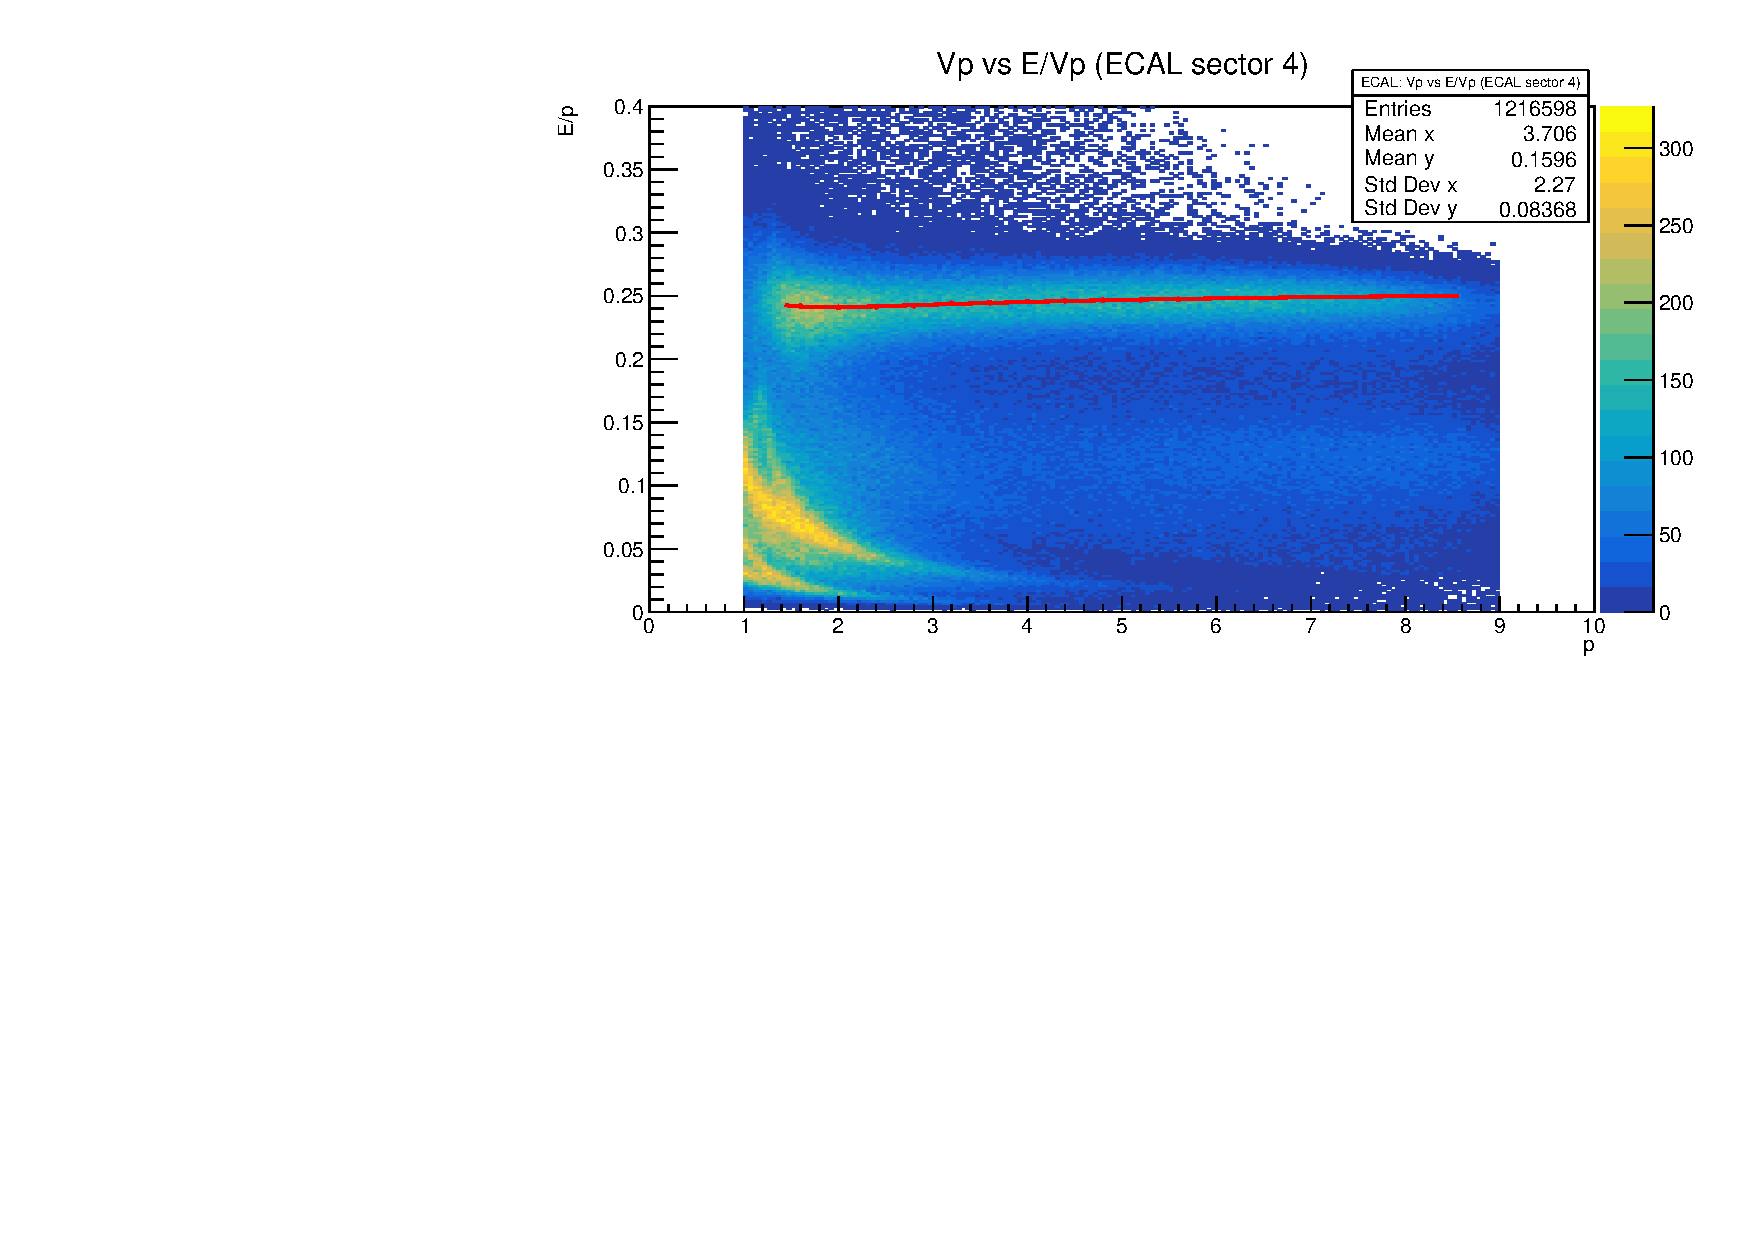
\includegraphics[width=\textwidth]{13data_analysis/img/30sf_2d_plot.pdf}}
        \caption[Calorimeters $p vs E/p$ plots]{A 2d plot showing momentum $p$ vs deposited energy divided by momentum $E/p$.
        The particle's deposited energy on all calorimeters is measured.
        Its momentum is obtained from tracking and the event builder.
        The fit follows the deposited energy of electrons to find their sampling fraction.
        Source: Own elaboration, using the \hyperlink{github.com/bleaktwig/clas12-rge-analysis}{clas12-rge-analysis} software.}
        \label{fig::sf_2d}
    \end{figure}

    Finally, the parameters of the fit are saved in plain text files, following the convention used in the CCDB.
    These parameters can be utilized later for particle identification purposes, specifically for electrons and photons.
    Furthermore, they are employed to determine the energy of electrons and photons since, as mentioned previously, not all of their energy is deposited in the calorimeters.

    % !TEX root = ../main.tex
\subsection{Acceptance Correction}
\label{ssec::acceptance_correction}
% --+ What is acceptance +------------------------------------------------------
    When discussing radiation detection, it is customary to distinguish between two types of efficiency: absolute efficiency and intrinsic detection efficiency.
    The former is defined as the fraction of events emitted by the source that are actually detected by the detector, expressed as
    \begin{equation*}
        \xi_\text{tot} = \frac{\text{events registered}}{\text{events emitted by source}}.
    \end{equation*}

    This efficiency is influenced by the detector's geometry and the probability of an interaction occurring within the detector.
    The total efficiency is also referred to as the detector acceptance.

    The total efficiency can be further decomposed into two components: the intrinsic efficiency, $\xi_{\text{int}}$, and the geometric efficiency, $\xi_{\text{geom}}$.
    The total efficiency is then given by
    \begin{equation*}
        \xi_\text{tot} = \xi_\text{int} \cdot \xi_\text{geom}.
    \end{equation*}

    The intrinsic efficiency represents the fraction of events that actually reach and are detected by the detector
    \begin{equation*}
        \xi_\text{int} = \frac{\text{events registered}}{\text{events impinging on detector}}.
    \end{equation*}

    This probability is dependent on the interaction cross-sections of the incident radiation with the detector medium.
    The intrinsic efficiency thus varies with the type of radiation, its energy, and the detector material \cite{leo1987}.

% --+ Acceptance correction through generation + simulation +-------------------
    Acceptance correction involves compensating for the total efficiency of the detector.
    To estimate this detector efficiency, a comparison is made between the total number of generated events, denoted as $N_\text{thrown}$, and the number of accepted events in a simulation of the detector, denoted as $N_\text{simul}$.
    This allows us to calculate an estimation of the detector efficiency, represented by $\tilde\xi_\text{tot}$, using
    \begin{equation*}
        \tilde\xi_\text{tot} = \frac{N_\text{simul}}{N_\text{thrown}}.
    \end{equation*}

    Naturally, the value of $\tilde\xi_\text{tot}$ is influenced by the accuracy and reliability of the event generator and simulation programs employed in the study.

% --+ Chosen bins +-------------------------------------------------------------
    The acceptance of the detector exhibits variations across the phase space of the kinematic variables.
    Therefore, in order to achieve accurate acceptance correction, the ratio $\tilde\xi_\text{tot}$ needs to be divided into bins in a five-dimensional space.
    These bins correspond to the five variables under investigation: $Q^2$, $\nu$, $z_h$, $p_T^2$, and $\phi_{PQ}$.
    To simplify the analysis process and facilitate interpretation of the results, it is advantageous to have bins of the same size for each variable.

    % TODO. I may need to update this list if I change these ranges in the future.
    \begin{itemize}
        \item
            $Q^2 = 4E_bE'\sin^2(\theta_C/2)$ is the 4-momentum transferred by the lepton probe in the lab frame, where $E_b$ is the beam energy, $E'$ is the scattered electron's energy, and $\theta_C$ is the polar angle of the scattered electron.
            The chosen bin edges are $1$, $2$, $3$, $4$, $5$, $6$, $7$, $8$, $9$, $10$, $11$ $\text{GeV}^2$.
        \item
            $\nu = E_v - E'$ is the energy transferred by the lepton probe in the lab frame.
            The chosen bin edges are $2$, $3$, $4$, $5$, $6$, $7$, $8$, $9$, and $10$ $\text{GeV}$.
        \item
            $z_h = E_h/\nu$ is the virtual photon energy fraction carried by the measured hadron, with $E_h$ being this hadron's energy.
            The chosen bin edges are $0$, $0.1$, $0.2$, $0.3$, $0.4$, $0.5$, $0.6$, $0.7$, $0.8$, $0.9$, and $1$.
        \item
            $p_T^2$ is the hadron's transverse momentum measured with respect to the virtual photon direction.
            The chosen bin edges are $0$, $0.2$, $0.4$, $0.6$, $0.8$, $1$, $1.2$, $1.4$, $1.6$, $1.8$, and $2$ $\text{GeV}^2$.
        \item
            $\phi_{PQ}$ is the angle between the leptonic plane -- the plane where the paths of the initial and scattered electrons lie -- and the hadronic plane, which contains the virtual photon and the measured hadron.
            The chosen bin edges are $-180$, $-140$, $-100$, $-60$, $-20$, $20$, $60$, $100$, $140$, and $180$ degrees.
    \end{itemize}

    To calculate the acceptance, 10 million events were initially generated in deep inelastic kinematics using LEPTO, a Monte Carlo generator specifically designed for deep inelastic lepton-nucleon scattering \cite{ingelman1997}.
    Subsequently, these events were simulated under the experimental conditions of the RG-F experiment in CLAS12 using \texttt{gemc}, which is the standard tool for CLAS12 event simulation \cite{ungaro2020gemc}.
    The simulation took into account a torus field polarity of $-1$ and a solenoid field polarity of $-0.745033$.

    Finally, the simulated events were reconstructed using \texttt{coatjava}, which is the standard tool for CLAS12 event offline reconstruction \cite{ziegler2020}.
    Further details regarding the offline reconstruction process can be found in Section \ref{sssec::offline_reconstruction}.
    The outcomes of the acceptance correction procedure are discussed in Section \ref{ssec::acceptance_correction_results}.

